\documentclass{article}
\usepackage[utf8]{inputenc}
\usepackage[a4paper, total={6in, 8in}]{geometry}
\usepackage{graphicx}
\title{CS 685 Assignment 1 Report}
\author{Gagandeep Mangat [20111019]}

\begin{document}
\maketitle

\section{Introduction}
The COVID data was accessed from the website \emph{https://api.covid19india.org/v4/data-all.json} which consisted of day-wise data of the districts and states tested, confirmed and deceased cases. District-wise data of the confirmed cases was extracted for a data range of 15th March, 2020 to 5th September, 2020. Along with the district-wise data, the state codes of the districts were also maintained. \\
The neighboring districts of all the districts were also maintained for the purpose of analysis and finding of hot spot and cold spot areas based on the cases of neighboring districts and other districts in the state respectively.\\
All the analysis was done based on week, month, and overall confirmed cases.  

\section{Analysis}
The time period of analysis consisted of a total of 175 days. A total of 58102 distinct date-wise and district-wise records of confirmed cases were found from the website. The data consisted of confirmed cases of 634 distinct districts. As of 2020, there are a total of 739 districts, which implied that either many districts did not have a COVID case for the time-period of analysis or they did not report their COVID cases. The states of Telengana, Sikkim, Manipur, Goa, and Assam did not report district-wise data of the confirmed cases and hence the districts of all these states present in the \emph{neighbor-districts.json} file were merged into a single district. Many other districts in the \emph{neighbor-districts.json} had to be renamed according to their names found from the portal districts. Also, all the Delhi and Mumbai districts present in the \emph{neighbor-districts.json} were merged to a single Delhi and Mumbai district. The redundant districts such as airport-quarantine, others, bsf-camp, etc were dropped. The total districts after all the pre-processing amounted to 627. \\

The total records of distinct date-wise and district-wise confirmed cases after the above steps were found to be 56802.\\
For a particular week, Pune had the highest number of cases with 25,111 confirmed cases during 30th August, 2020 to 5th Septemeber, 2020 followed by Delhi with 23,442 confirmed cases during 21st June, 2020 to 27th June, 2020.\\
Pune also had the most number of confirmed cases in a month with a total of 85,874 confirmed cases for the month of August.\\
For the overall time period of analysis, Pune again dominated the charts with a total of 1,93,507 confirmed cases, followed by Delhi with 188186, Mumbai with 1,48,305 , Bengaluru Urban with 1,44,628 and Thane with 1,40,253 confirmed cases.\\
\\
\\
The hot spots and cold spots are found on the basis of either the neighborhood data of a district or the data of other districts in the state of that district. \\
Finding hot spots on the basis of neighborhood data would essentially mean that the particular district has a comparatively high number of cases than its neighboring districts. While a cold spot would signify the lesser number of cases of that district compared to the other neighboring districts.\\
On the other hand, finding hot spots on the basis of state data would mean that the particular district which is the hot spot has a comparatively high number of cases than all the other districts in its state. Cold spots would signify the district has a fewer proportion of cases of the entire state.\\ \\
The top 5 hot spots and cold spots for the overall time-period of analysis according to state data are Puducherry, Bengaluru Urban, Chennai, Raipur, and Patna \& Diu, Krishna, Lahaul and Spiti, Vizianagaram, and Wayanad respectively. \\

The top 5 hot spots and cold spots for the overall time-period of analysis according to neighborhood data are Bengaluru Urban, Assam District, Bhopal, Surat and Delhi \& Upper Dibang Valley, South Tripura, Unokoti, Karaikal, and Mahe respectively.\\

The number of cases in every state were analysed and Maharashtra dominated the charts with an astonishing more than 8,00,000 cases in the time period followed by Andhra Pradesh at 4,83,339 and Tamil Nadu at 4,05,675. \\
The least hit states were Mizoram, Sikkim, Daman and Diu, Ladakh, Meghalya, Nagaland and Arunachal Pradesh with less than 5,000 cases reported in the time period of analysis. \\

The state information for districts was retrieved from the portal \emph{data-all.json} file while finding the number of cases of each district. The information was stored in a dataframe stored as \emph{cases-all-detailed.csv}, which was then used to find the further computations requiring state wise information for a district. \\ \\
The following map chart summarizes the cases in the states of India. \\

\begin{figure}
  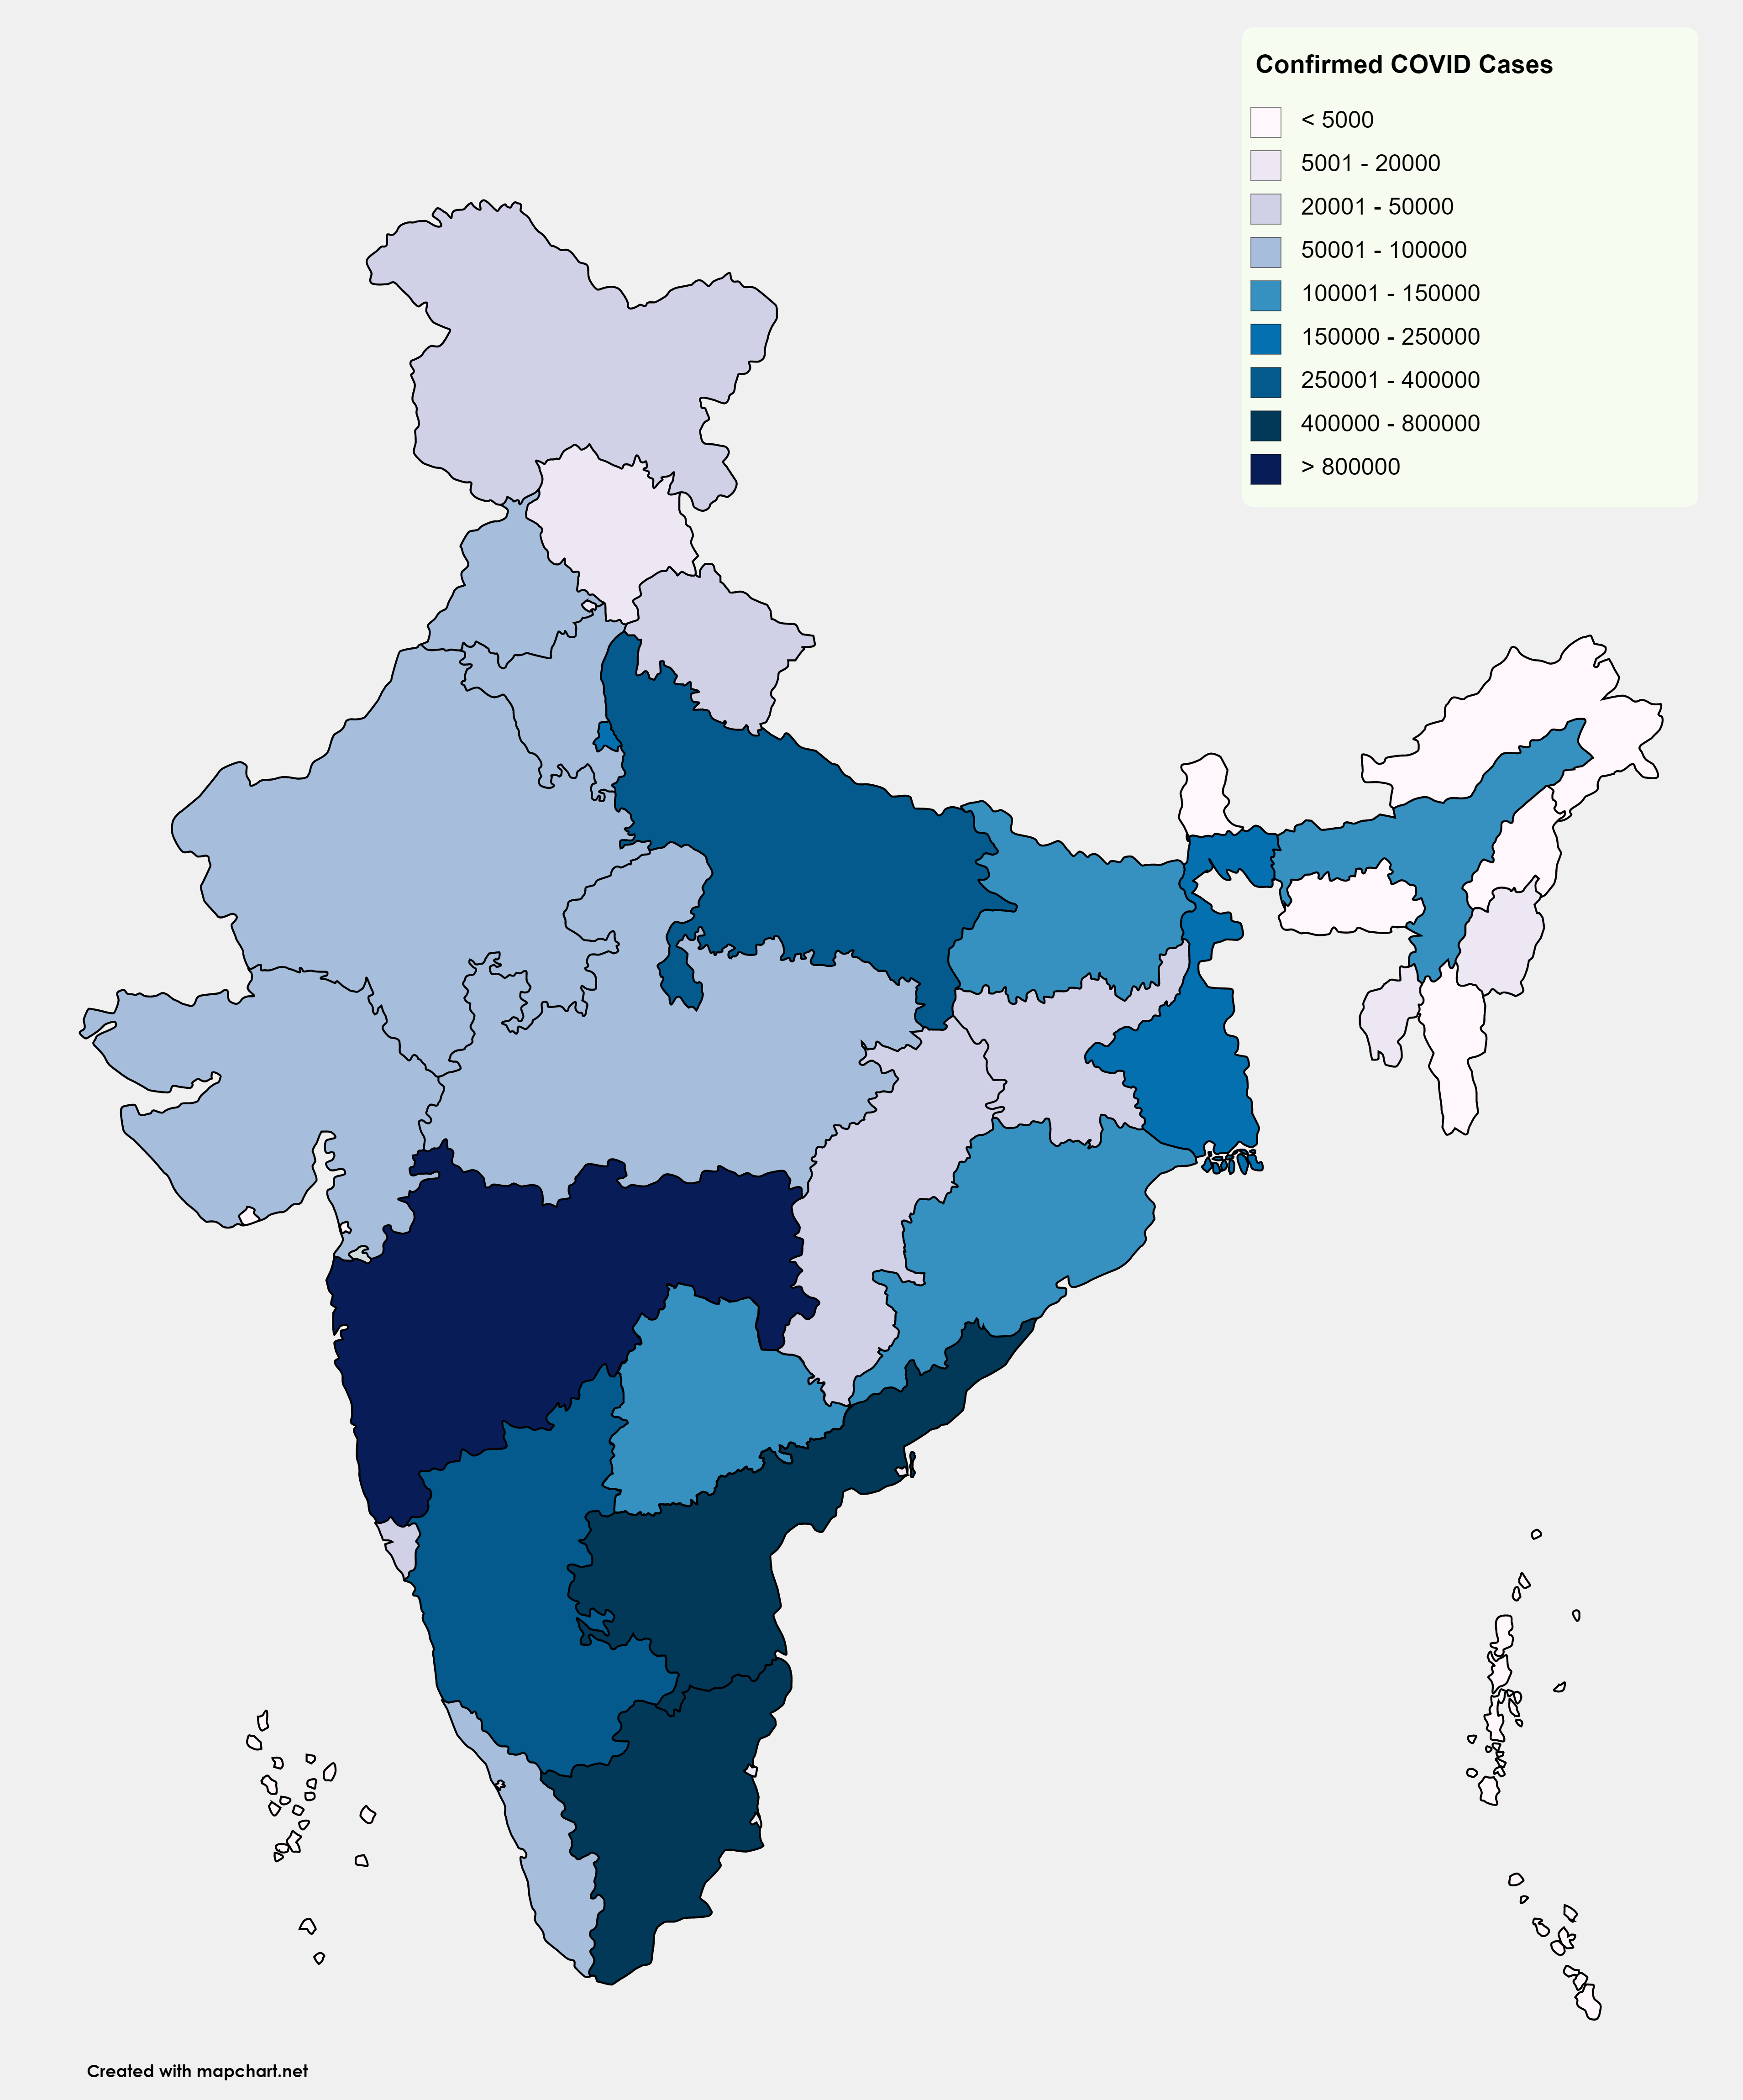
\includegraphics[width=\textwidth,height=\textheight,keepaspectratio]{images/chartmap.png}
  \caption{State-wise COVID cases chart}
\end{figure}




\end{document}

